\chapter{Feynman diagrams}
\section{a baby problem}
\begin{itemize}
	\item 考虑如下积分,
	\begin{equation} \label{4.1.1}
		Z(J) = \int_{- \infty}^{+ \infty} dq \, e^{- \frac{1}{2} m^2 q^2 - \frac{\lambda}{4!} q^4 + J q}
	\end{equation}
	
	\item 把 integrand 对 $\lambda$ 展开, 并将 $q$ 用 $\frac{\partial}{\partial J}$ 替代, 得到,
	\begin{align}
		Z(J) &= e^{- \frac{\lambda}{4!} (\frac{\partial}{\partial J})^4} \int_{- \infty}^{+ \infty} dq \, e^{- \frac{1}{2} m^2 q^2 + J q} \notag \\
		&= \sqrt{\frac{2 \pi}{m^2}} e^{- \frac{\lambda}{4!} (\frac{\partial}{\partial J})^4} e^{\frac{J^2}{2 m^2}} \label{4.1.2}
	\end{align}
	后面的计算中忽略 $Z(J = 0, \lambda = 0)$.
	
	\item 每个 vertex 带有 $- \lambda$, 每个 line 带有 $\frac{1}{m^2}$, 剩下的系数通过展开项算, 如下 (numerical factors 怎么算 \textcolor{red}{(?)}),
	
	\begin{figure}[H]
		\centering
		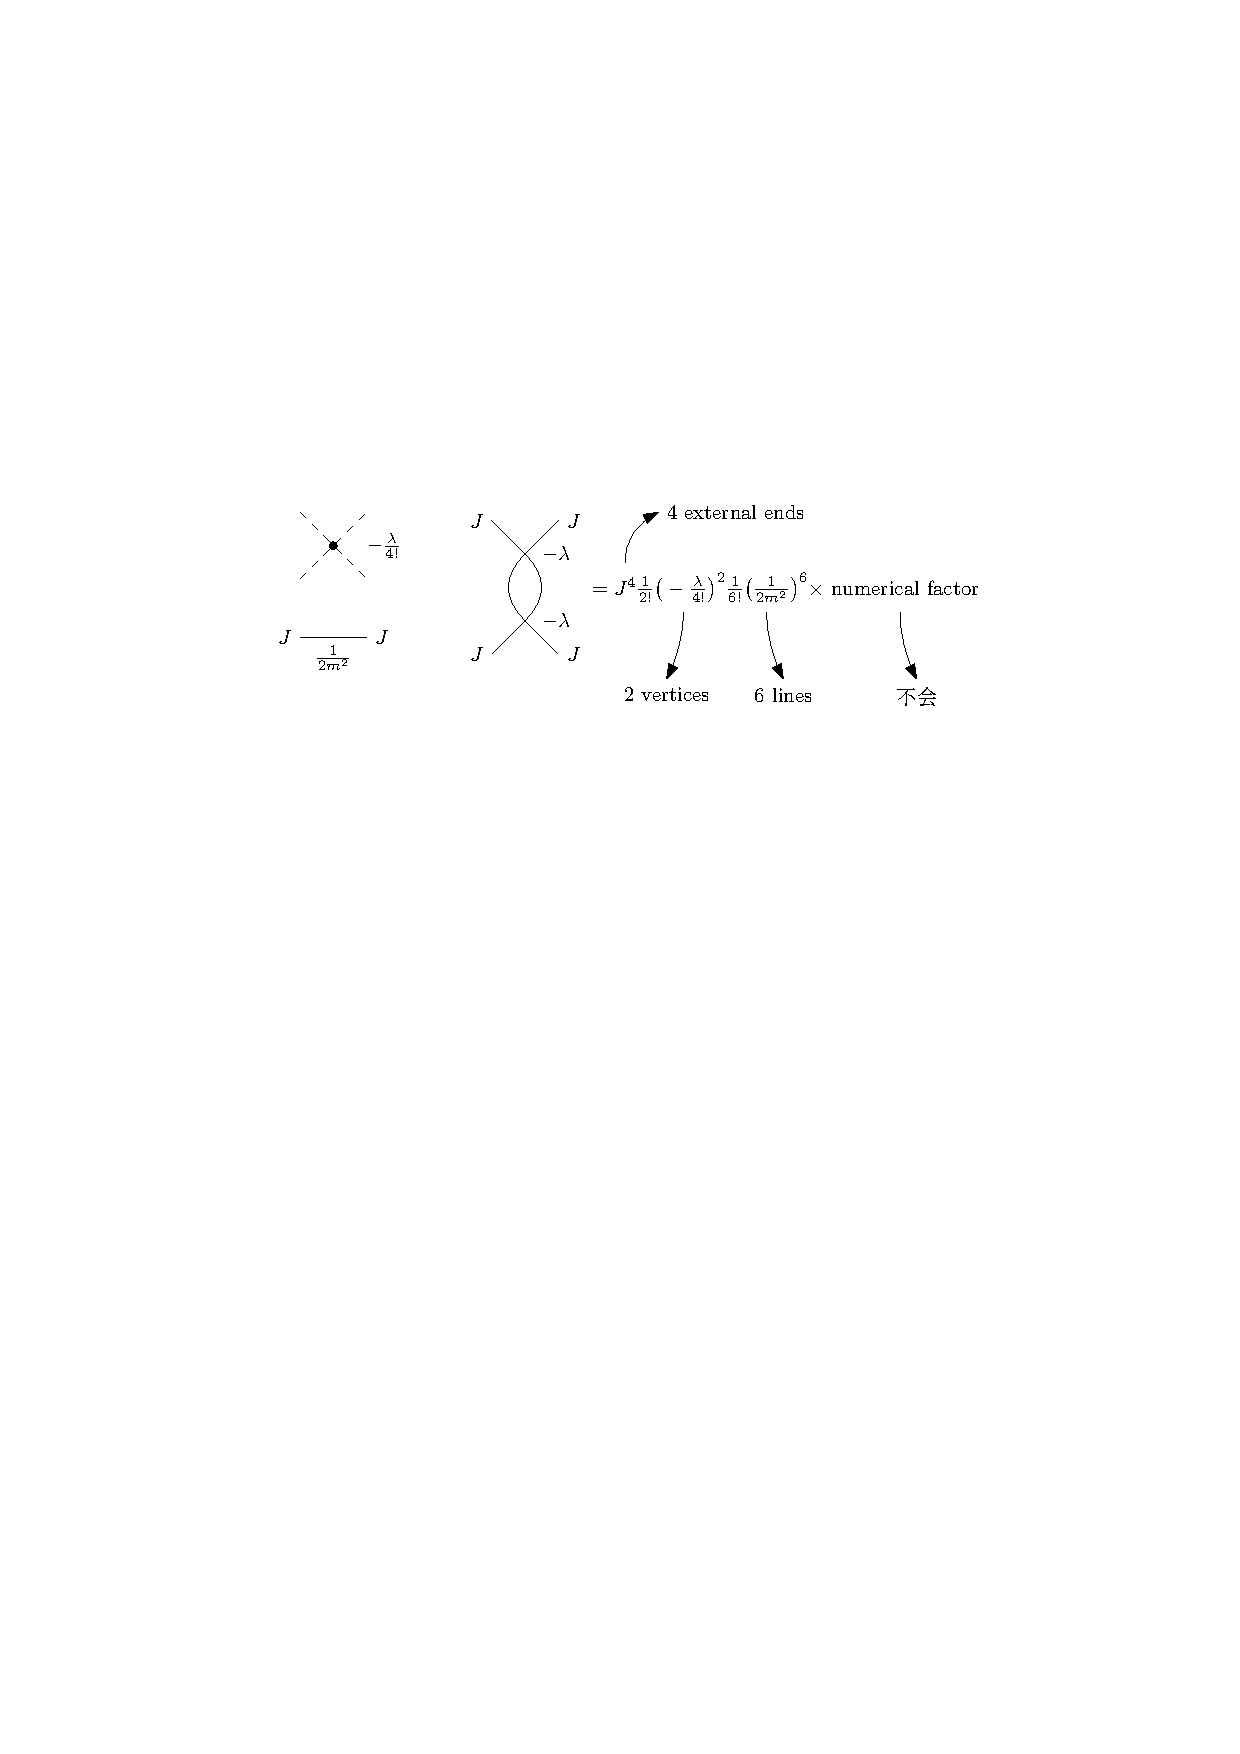
\includegraphics[scale=1]{figures/a baby problem - Feynman diagram.pdf}
	\end{figure}
	
	\begin{tcolorbox}[title=calculation:]
		在这里计算 $\lambda J^4$ 项,
		\begin{equation}
			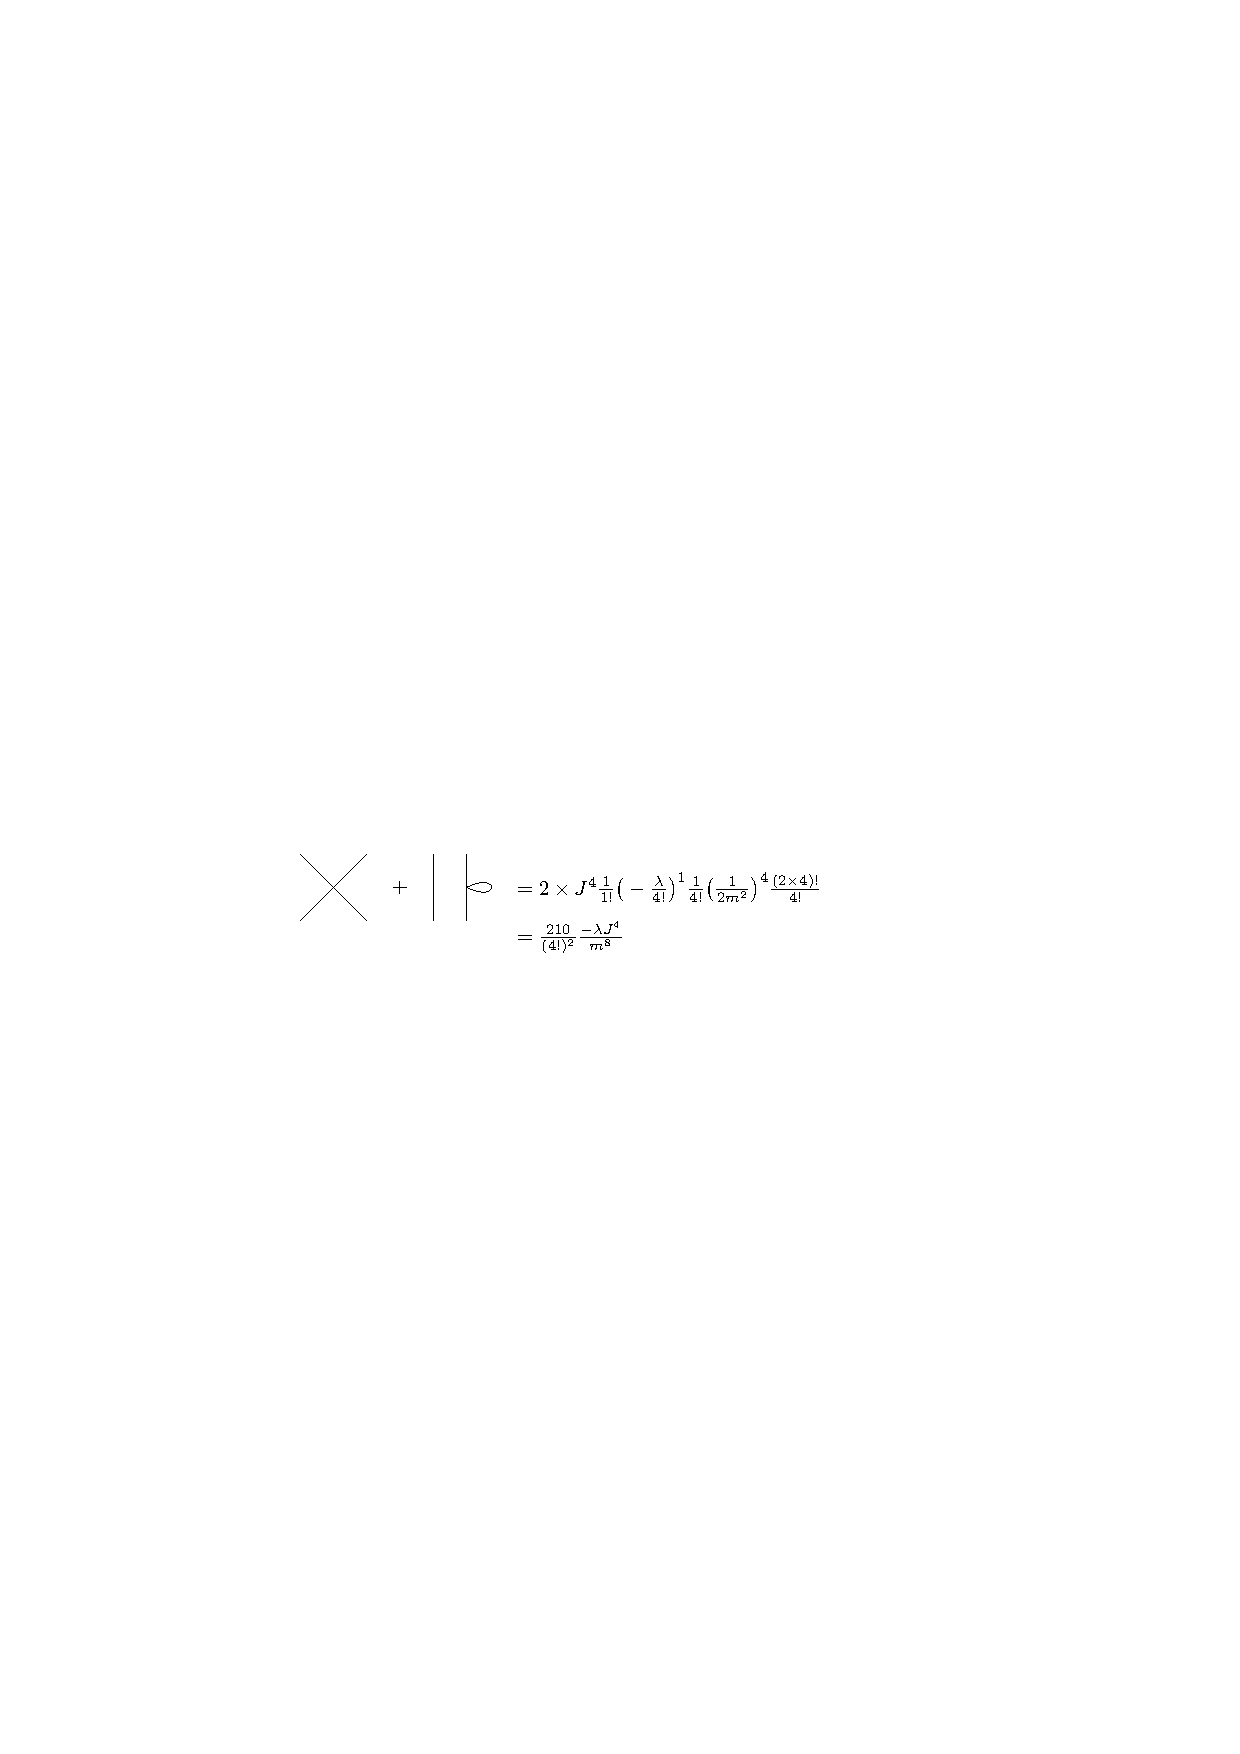
\includegraphics[scale=1]{figures/a baby problem - lambda J^4 terms.pdf}
		\end{equation}
		但是直接计算 \eqref{4.1.2} 的展开项, 得到的结果与 \eqref{4.1.5} 一样.
	\end{tcolorbox}
\end{itemize}

\subsection{Wick contraction and Green's functions}
\begin{itemize}
	\item 把积分 \eqref{4.1.1} 对 $J$ 展开,
	\begin{equation}
		Z(J) = \sum_{n = 0}^\infty \frac{1}{n!} J^n \underbrace{\int_{- \infty}^{+ \infty} dq \, e^{- \frac{1}{2} m^2 q^2 - \frac{\lambda}{4!} q^4} q^n}_{= Z(0, 0) G^{(n)}}
	\end{equation}
	其中 Green's function $G^{(n)}$ 对 $\lambda$ 展开后, 可以用 Wick contraction 计算, 见 \eqref{B.1.5}.
	
	\begin{tcolorbox}[title=calculation:]
		计算 $\lambda J^4$ 项, 它来自 $G^{(4)}$ 对 $\lambda$ 展开的一阶项,
		\begin{align}
			- \frac{\lambda}{4!} \int dq \, e^{- \frac{1}{2} m^2 q^2} q^8 &= - \frac{\lambda}{4!} \braket{q^8} \notag \\
			&= - \frac{\lambda}{4!} \sum_{\text{Wick}} \Big( \frac{1}{m^2} \Big)^4 \notag \\
			&= - \frac{\lambda}{4!} \frac{7 \times 5 \times 3 \times 1}{m^8} \label{4.1.5}
		\end{align}
		所以 $\lambda J^4$ 项等于 $\frac{105}{(4!)^2} \frac{- \lambda J^4}{m^8}$.
	\end{tcolorbox}
\end{itemize}

\subsection{connected vs. disconnected}
\begin{itemize}
	\item 考虑,
	\begin{equation}
		Z(J, \lambda) = Z(J = 0, \lambda) e^{W(J, \lambda)}
	\end{equation}
	其中 $Z(J = 0, \lambda)$ 由 diagrams with no external source $J$ 组成, 而 $W(J, \lambda)$ 则由 connected diagrams 组成 \textcolor{red}{(?)}.
	
	\item 我们希望计算的是 $W$, 而不是 $Z$ \textcolor{red}{(?)}.
\end{itemize}

\section{a child problem}
\begin{itemize}
	\item 考虑如下积分,
	\begin{equation}
		Z(J) = \int dq_1 \cdots dq_N \, e^{- \frac{1}{2} q^T \cdot A \cdot q - \frac{\lambda}{4!} q^4 + J^T \cdot q}
	\end{equation}
	其中 $q^4 = \sum_i q_i^4$.
	
	\item 对 $\lambda$ 展开并把 $q$ 替换为 $\frac{\partial}{\partial J}$, 得到,
	\begin{equation}
		Z(J) = \sqrt{\frac{(2 \pi)^N}{\det A}} e^{- \frac{\lambda}{4!} (\frac{\partial}{\partial J})^4} e^{\frac{1}{2} J^T \cdot A^{- 1} \cdot J}
	\end{equation}
	其中 $\big( \frac{\partial}{\partial J} \big)^4 = \sum_i \big( \frac{\partial}{\partial J_i} \big)^4$.
\end{itemize}

\subsection{\texorpdfstring{$n$}{n}-point Green's function}
\begin{itemize}
	\item 对 $J$ 展开获得带 Green's function 的表达式,
	\begin{equation}
		Z(J) = \sum_{n = 0}^\infty \frac{1}{n!} \sum_{i_1 = 1}^N \cdots \sum_{i_n = 1}^N J_{i_1} \cdots J_{i_n} \underbrace{\int dq_1 \cdots dq_N \, e^{- \frac{1}{2} q^T \cdot A \cdot q - \frac{\lambda}{4!} q^4} q_{i_1} \cdots q_{i_n}}_{= Z(0, 0) G^{(n)}_{i_1 \cdots i_n}}
	\end{equation}
	其中 $G^{(n)}_{i_1 \cdots i_n}$ 称为 $n$-point Green's function.
	
	\begin{tcolorbox}[title=Taylor expansion:]
		多元函数的 Taylor 展开如下,
		\begin{align}
			f(x_1, \cdots, x_N) &= \sum_{n_1 = 0}^\infty \cdots \sum_{n_N = 0}^\infty \frac{x_1^{n_1}}{n_1 !} \cdots \frac{x_N^{n_N}}{n_N !} \frac{\partial^{n_1}}{\partial x_1^{n_1}} \cdots \frac{\partial^{n_N}}{\partial x_N^{n_N}} f(x = 0) \notag \\
			&= \sum_{n = 0}^\infty \frac{1}{n!} \sum_{i_1 = 1}^N \cdots \sum_{i_n = 1}^N x_{i_1} \cdots x_{i_n} \frac{\partial}{\partial x_{i_1}} \cdots \frac{\partial}{\partial x_{i_N}} f(x = 0)
		\end{align}
		这两种求和方法, $x_1^{n_1} \cdots x_N^{n_N}$ 项的 numerical factor 都等于,
		\begin{equation}
			\frac{1}{n!} \times \frac{n!}{n_1 ! \cdots n_N !} = \frac{1}{n_1 ! \cdots n_N !}
		\end{equation}
		其中 $n = n_1 + \cdots + n_N$.
	\end{tcolorbox}
	
	\item 在 $\lambda = 0$ 时, $2$-point Green's function 就是 propagator,
	\begin{align}
		G^{(2)}_{i j}(\lambda = 0) &= \frac{1}{Z(0, 0)} \int dq_1 \cdots dq_N \, e^{- \frac{1}{2} q^T \cdot A \cdot q} q_i q_j \notag \\
		&= \frac{\partial}{\partial J_i} \frac{\partial}{\partial J_j} e^{\frac{1}{2} J^T \cdot A^{- 1} \cdot J} \Big|_{J = 0} = A^{- 1}_{i j}
	\end{align}
	
	\item 来计算 $2, 3, 4$-point Green's functions,
	\begin{align}
		G^{(2)}_{i j} =& A^{- 1}_{i j} - \frac{\lambda}{4!} \sum_m (3 A^{- 1}_{m m} A^{- 1}_{m m} A^{- 1}_{i j} + 12 A^{- 1}_{m m} A^{- 1}_{m i} A^{- 1}_{m j}) + O(\lambda^2) \\
		G^{(3)}_{i j k} =& 0 \\
		G^{(4)}_{i j k l} =& A^{- 1}_{i j} A^{- 1}_{k l} + A^{- 1}_{i k} A^{- 1}_{j l} + A^{- 1}_{i l} A^{- 1}_{j k} \notag \\
		& - \frac{\lambda}{4!} \sum_m (A^{- 1}_{m m} A^{- 1}_{m m} A^{- 1}_{i j} A^{- 1}_{k l} + \cdots + 4! A^{- 1}_{i m} A^{- 1}_{j m} A^{- 1}_{k m} A^{- 1}_{l m}) + O(\lambda^2)
	\end{align}
	
	\begin{tcolorbox}[title=calculation:]
		$2$-point Green's function 计算如下,
		\begin{align}
			G^{(2)}_{i j} &= \frac{1}{Z(0, 0)} \int dq_1 \cdots dq_N \, e^{- \frac{1}{2} q^T \cdot A \cdot q} \Big( 1 - \frac{\lambda}{4!} q^4 + O(\lambda^2) \Big) q_i q_j \notag \\
			&= A^{- 1}_{i j} - \frac{\lambda}{4!} \braket{q^4 q_i q_j} + O(\lambda^2) \notag \\
			&= A^{- 1}_{i j} - \frac{\lambda}{4!} \sum_m (3 A^{- 1}_{m m} A^{- 1}_{m m} A^{- 1}_{i j} + 12 A^{- 1}_{m m} A^{- 1}_{m i} A^{- 1}_{m j}) + O(\lambda^2)
		\end{align}
		$3$-point Green's function 计算如下,
		\begin{equation}
			G^{(32)}_{i j k} = \frac{1}{Z(0, 0)} \int dq_1 \cdots dq_N \, e^{- \frac{1}{2} q^T \cdot A \cdot q} \Big( 1 - \frac{\lambda}{4!} q^4 + O(\lambda^2) \Big) q_i q_j q_k = 0
		\end{equation}
		$4$-point Green's function 计算如下,
		\begin{align}
			G^{(4)}_{i j k l} &= \frac{1}{Z(0, 0)} \int dq_1 \cdots dq_N \, e^{- \frac{1}{2} q^T \cdot A \cdot q} \Big( 1 - \frac{\lambda}{4!} q^4 + O(\lambda^2) \Big) q_i q_j q_k q_l \notag \\
			&= A^{- 1}_{i j} A^{- 1}_{k l} + A^{- 1}_{i k} A^{- 1}_{j l} + A^{- 1}_{i l} A^{- 1}_{j k} - \frac{\lambda}{4!} \braket{q^4 q_i q_j q_k q_l} + O(\lambda^2)
		\end{align}
	\end{tcolorbox}
\end{itemize}

\section{perturbative field theory}
\begin{itemize}
	\item 做如下替换即可,
	\begin{equation}
		\begin{dcases}
			A \mapsto - i (\partial^2 - m^2) \\
			J \mapsto i J
		\end{dcases}
	\end{equation}
	
	\item $\phi^4$ theory 的路径积分,
	\begin{align}
		Z(J) &= \int D\phi \, e^{i \int d^d x \, (\frac{1}{2} \phi (\partial^2 - m^2) \phi - \frac{\lambda}{4!} \phi^4 + J(x) \phi(x))} \\
		&= Z(0, 0) e^{- i \frac{\lambda}{4!} \int d^d z \, (\frac{\delta}{i \delta J(z)})^4} e^{- \frac{i}{2} \int d^d x d^d y \, J(x) D(x - y) J(y)}
	\end{align}
	这种方法称作 \textbf{'Schwinger way'}, 其中 $D(x - y)$ 是自由场的 propagator, 见 \eqref{1.2.1}.
	
	\item 同样, 对 $J$ 展开得到含 Green's functions 的表达式,
	\begin{equation}
		\frac{Z(J)}{Z(0, 0)} = \sum_{n = 0}^\infty \frac{i^n}{n!} \int d^d x_1 \cdots d^d x_n \, J(x_1) \cdots J(x_n) G^{(n)}(x_1, \cdots, x_n)
	\end{equation}
	这种方法称作 \textbf{'Wick way'}, 其中,
	\begin{equation}
		G^{(n)}(x_1, \cdots, x_n) = \frac{1}{Z(0, 0)} \int D\phi \, e^{i \int d^d x \, (\frac{1}{2} \phi (\partial^2 - m^2) \phi - \frac{\lambda}{4!} \phi^4)} \phi(x_1) \cdots \phi(x_n)
	\end{equation}
	有时 $Z(J)$ 被称为 generating functional, 因为它能生成 Green's functions.
\end{itemize}

\subsection{collision between particles}
\begin{itemize}
	\item 
\end{itemize}
